\documentclass[Bachelorarbeit.tex]{subfiles}
\begin{document}

\chapter{Prototyp}
\label{bilderPrototyp}

\begin{figure}[h]
\centering
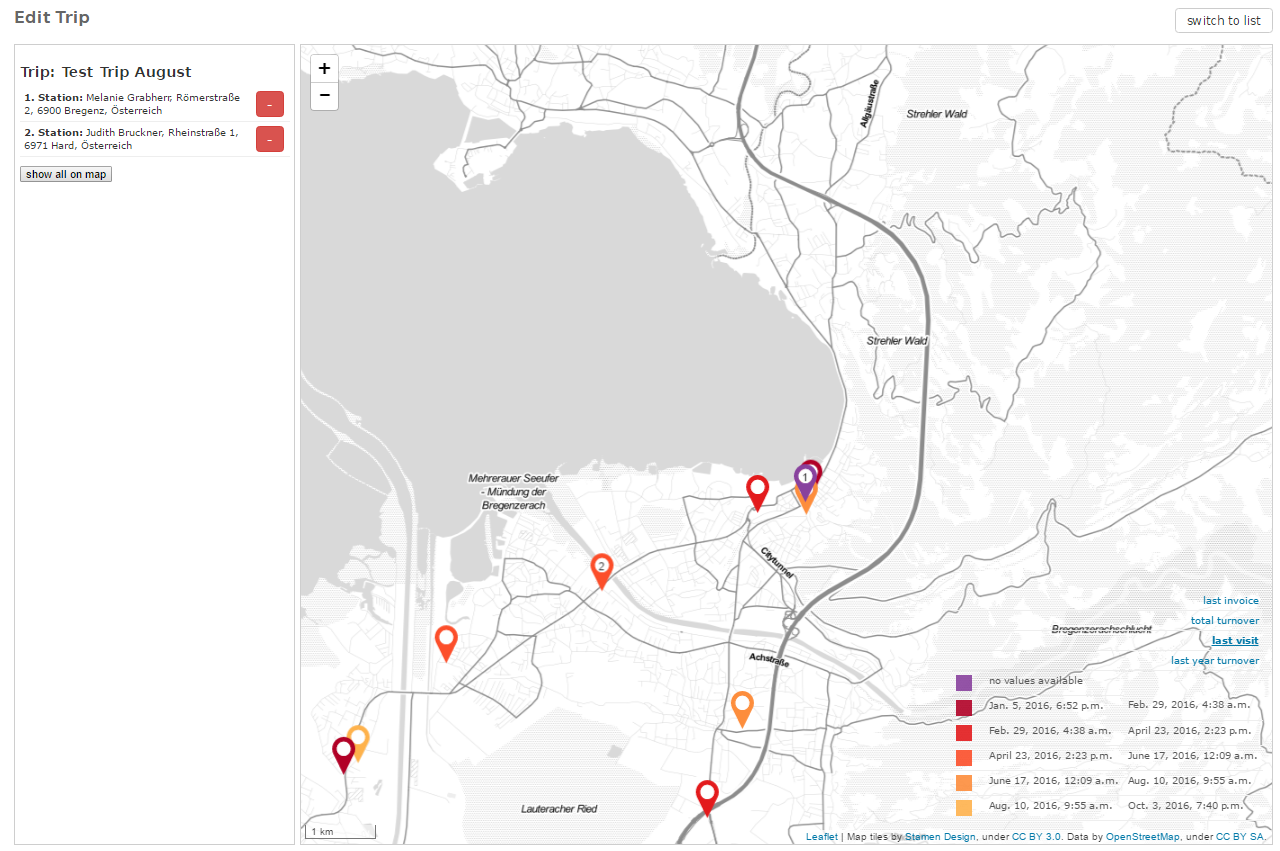
\includegraphics[width=1\linewidth]{img/Prototyp/mapView}
\caption[Prototyp mit Kartenansicht]{Prototyp mit Kartenansicht. Quelle: eigene Ausarbeitung}
\label{fig:mapView}
\end{figure}

\begin{figure}[h]
\centering
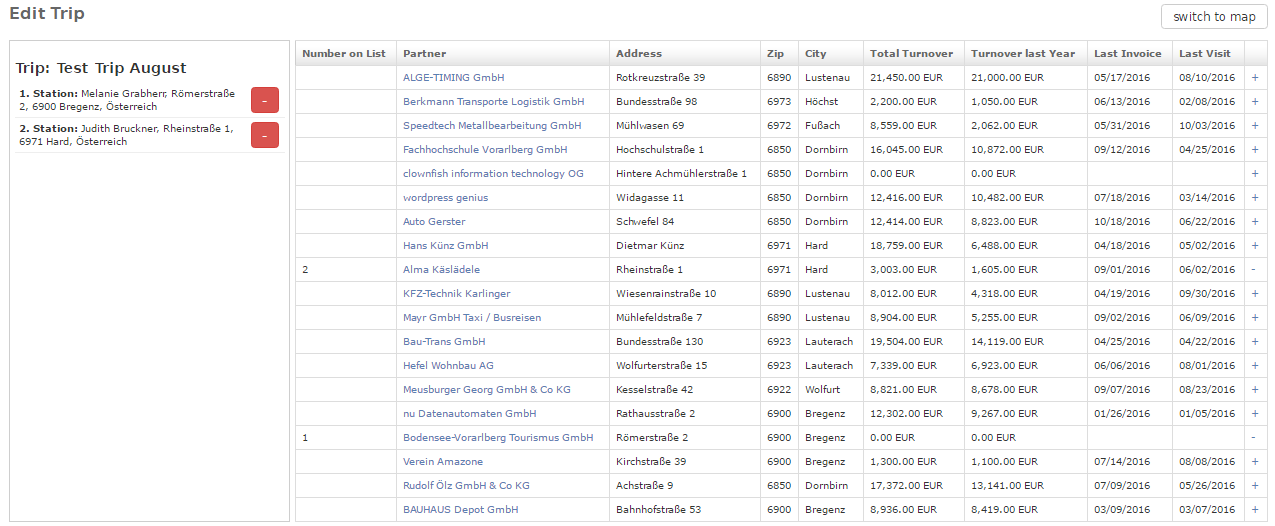
\includegraphics[width=1\linewidth]{img/Prototyp/listView}
\caption[Prototyp mit Listenansicht]{Prototyp mit Listenansicht. Quelle: eigene Ausarbeitung.}
\label{fig:listView}
\end{figure}

\begin{figure}[h]
\centering
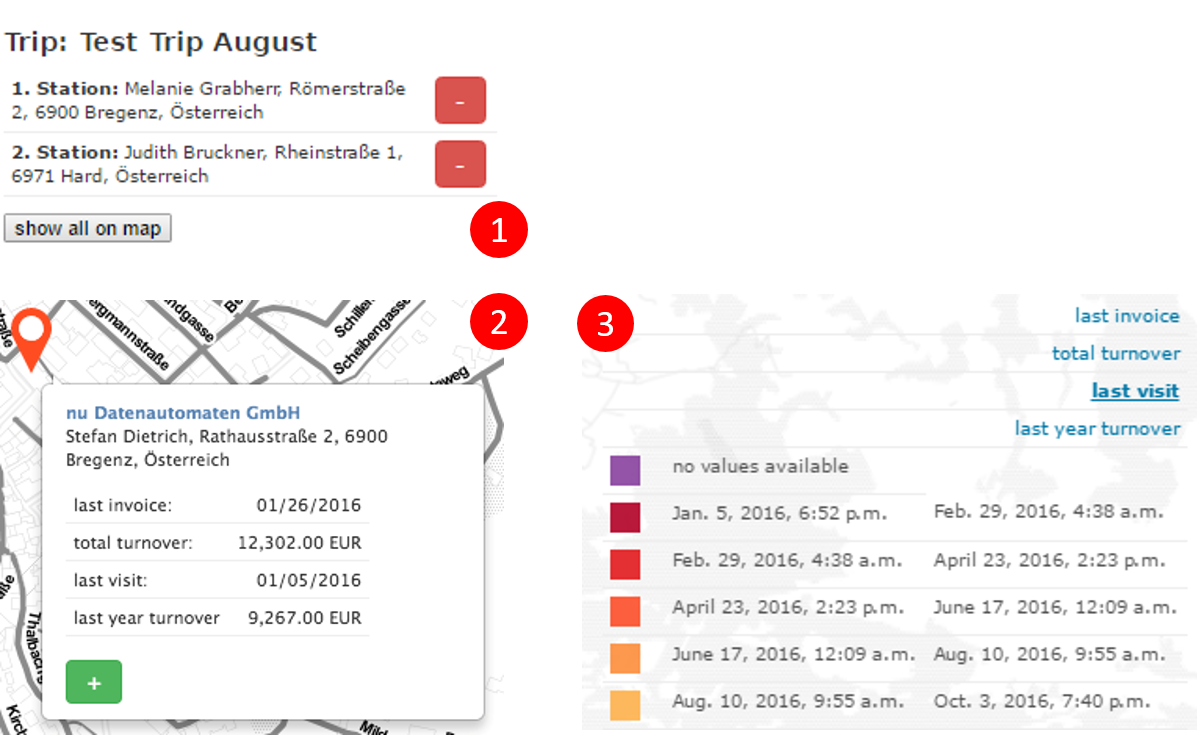
\includegraphics[width=1\linewidth]{img/Prototyp/Details}
\caption[Prototyp: Detailansichten]{Prototyp: Detailansichten. Markierung 1: Trip Liste, Markierung 2: Popup in der Kartenansicht, Markierung 3: Rank-Bereich in der Kartenansicht. Quelle: eigene Ausarbeitung.}
\label{fig:Details}
\end{figure}

\end{document}